\lab{Изучение плазмы газового разряда в неоне}

%Контрольные вопросы так же стоят после теоретического минимума. В этой лабе и
% лабе 3.5.2 их не было. Тем не менее, можно в эти лабы добавить вопросы 1, 3--5,
% 7.

\aim{изучение вольт-амперной характеристики тлеющего разряда; изучение свойств
плазмы методом зондовых характеристик.}

\equip{стеклянная газоразрядная трубка, наполненная изотопом неона,
высоковольтный источник питания, источник питания
постоянного тока, делитель напряжения, резистор, потенциометр, амперметры,
вольтметры, переключатели.}

Перед выполнением работы необходимо ознакомиться с разделами
\ref{sec:plasma}, \ref{sec:single} и \ref{sec:double} теоретического введения.
Подробное описание свойств тлеющего разряда можно найти в Приложении.

Схема установки для исследования плазмы газового разряда в неоне представлена на
рис.~\figref{Neon gas discharge}. Стеклянная газоразрядная
трубка имеет холодный (ненакаливаемый) полый катод, три анода и
\important{геттерный узел}~--- стеклянный баллон, на
внутреннюю поверхность которого напылена газопоглощающая плёнка
(\important{геттер}). Трубка наполнена изотопом неона
$^{22}$Ne при давлении 2~мм~рт. ст. Катод и один из анодов (I или II) с~помощью
переключателя $\text{П}_1$ подключаются через
балластный резистор~$R_\text{б}$ ($\sim500$ кОм) к~регулируемому высоковольтному
источнику питания (ВИП) с~выходным
напряжением до нескольких киловольт.

\begin{figure}[h!]
    \centering
	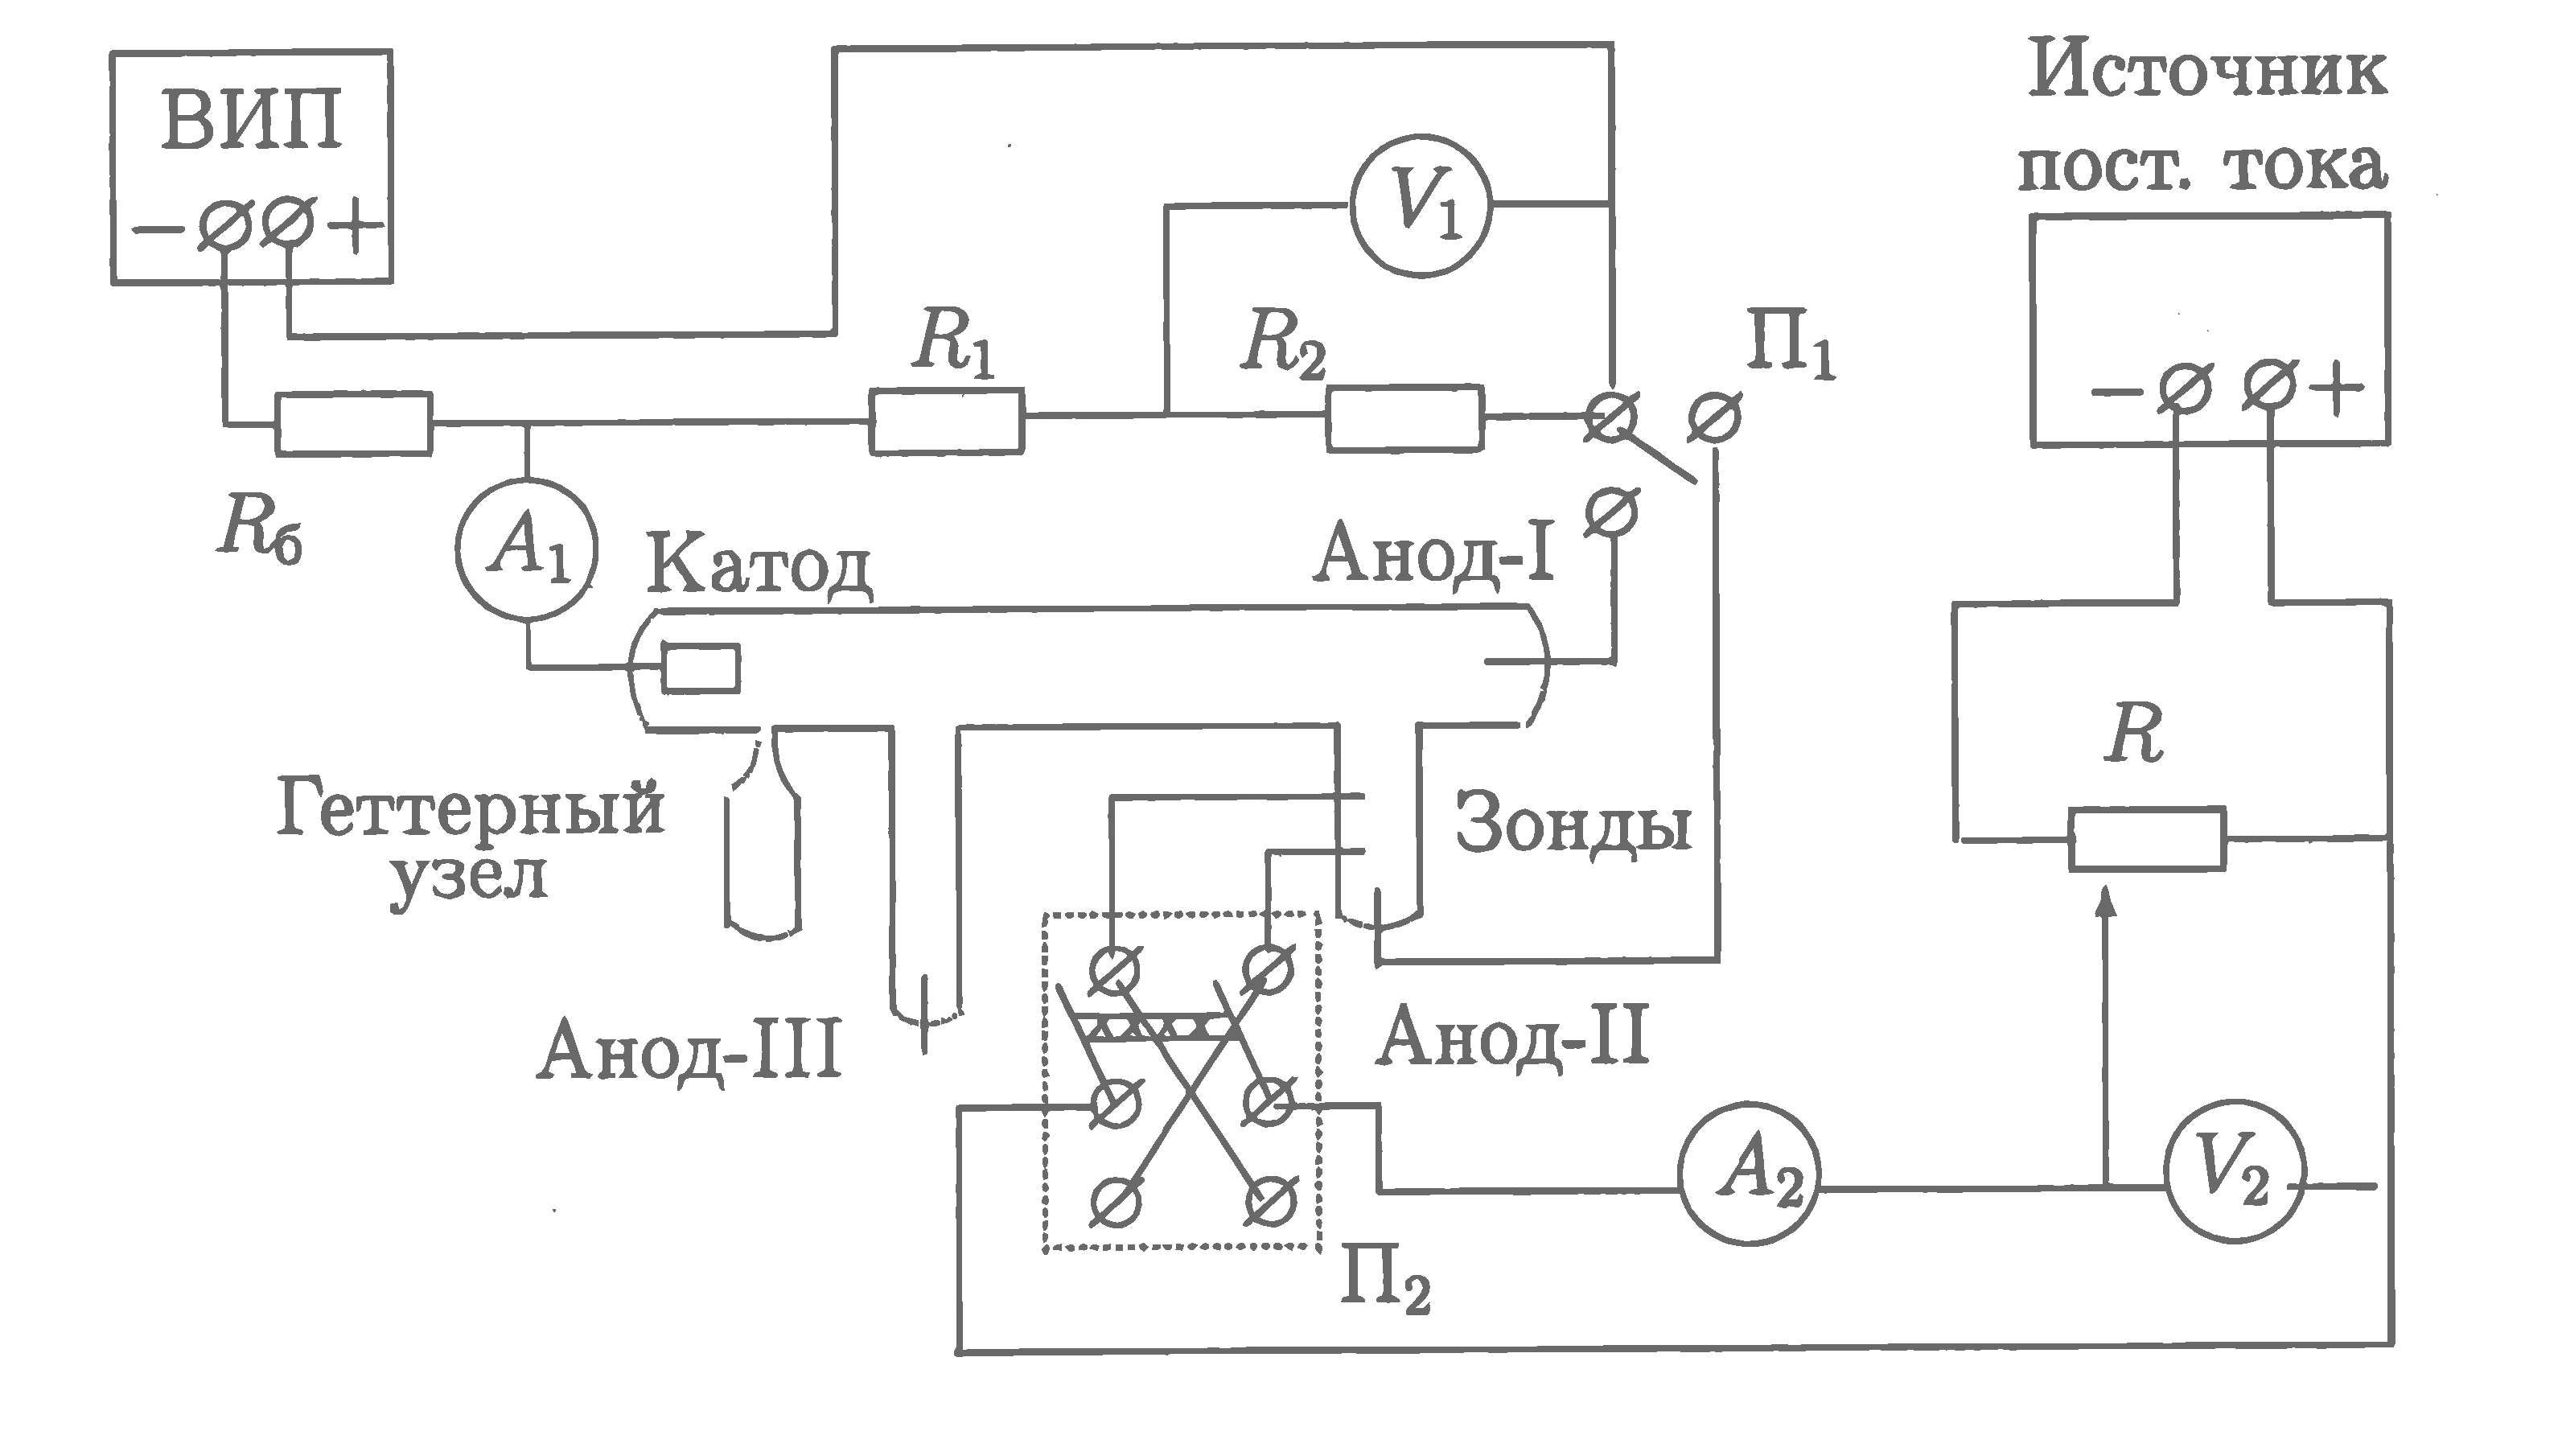
\includegraphics[width = 0.9\textwidth]{Chapter_5/3_5_1.eps}
	\caption{Схема установки для исследования газового разряда}
	\figmark{Neon gas discharge}
\end{figure}

При подключении к ВИП анода-I между ним и катодом возникает газовый разряд. Ток
разряда измеряется миллиамперметром
$A_1$, а падение напряжения на разрядной трубке~--- цифровым вольтметром
$V_{1}$, подключённым к трубке через
высокоомный (несколько десятков МОм) делитель напряжения с коэффициентом
$(R_1+R_2)/R_2$.

При подключении к ВИП анода-II разряд возникает в~проcтранстве между катодом и
анодом-II, где находится двойной зонд,
используемый для диагностики плазмы положительного столба. Зонды изготовлены из
молибденовой проволоки диаметром
$d$ и имеют длину~$l$. Они подключены к источнику питания через
потенциометр~$R$. Переключатель
$\text{П}_2$ позволяет изменять полярность напряжения на зондах. Величина
напряжения на зондах изменяется с~помощью дискретного
переключателя <<$V$>> выходного напряжения источника питания и потенциометра
$R$, а измеряется вольтметром~$V_2$. Для
измерения зондового тока используется микроамперметр~$A_2$.
Анод-III в нашей работе не используется.


\begin{lab:task}

В работе предлагается снять вольт-амперную характеристику тлеющего разряда и
зондовые характеристики при разных токах
разряда и по результатам измерений рассчитать концентрацию и температуру
электронов в плазме, степень ионизации,
плазменную частоту и дебаевский радиус экранирования.



\tasksection{Вольт-амперная характеристика разряда}

\begin{enumerate}
\item Установите переключатель~$\text{П}_1$ в положение <<Анод-I>> и подготовьте
приборы к работе согласно техническому описанию, которое находится в
лаборатории. Плавно увеличивая выходное напряжение ВИП, определите напряжение
зажигания разряда (показания вольтметра~$V_{1}$ перед зажиганием).

\item С помощью вольтметра~$V_{1}$ и амперметра~$A_{1}$ снимите вольт-амперную
характеристику разряда $U_{1}=f(I_\text{р})$. Ток разряда~$I_\text{р}$ изменяйте
в диапазоне, указанном в описании работы в лаборатории (при больших токах может
сгореть сопротивление).

\end{enumerate}

\tasksection{Зондовые характеристики}

\begin{enumerate}
\item Уменьшите напряжение ВИП до нуля, переведите переключатель~$\text{П}_1$
в~положение <<Анод-II>> и подготовьте приборы~$\text{П}_{2}$, $V_{2}$ и~$A_{2}$
к работе согласно техническому описанию, которое находится в лаборатории.

\item Плавно увеличивайте напряжение ВИП до возникновения разряда. Установите
значение разрядного тока~$I_\text{р}$ согласно техническому описанию.
Подготовьте к работе источник питания. После этого при помощи
потенциометра~$R$ установите на зонде максимальное напряжение $U_{2 max}$.

\item Снимите вольт-амперную характеристику двойного зонда $I_{2}(U_{2})$
(в диапазоне от~$-U_{2 \rm max}$ до~$U_{2 \rm max}$) при фиксированном токе~$I_\text{p}$
согласно описанию работы в лаборатории.

\item Повторите измерения при другой полярности (переключатель~$\text{П}_2$).
Менять полярность подключения зондов можно только при \important{нулевом токе},
поддерживая при этом величину тока разряда~$I_\text{p}$ в трубке.

Записывая результаты в таблицу, одновременно стройте приближенный график
$I(U)$  в тетради в интервале от $-U_{2 \rm max}$ до~$U_{2 \rm max}$. Отцентрируйте
кривую: проведите ось абсцисс на уровне $I=\sum \Delta I/2$, восстановите ось
ординат из точки пересения кривой с новой осью абсцисс. Убедитесь, что можно
провести асимптоты к участкам кривой при больших напряжениях. Если точек мало~---
проведите дополнительные измерения.

\item Снимите зондовые характеристики при токах разряда, равных~3 и 1,5~мА.
\end{enumerate}

\tasksection{Обработка результатов}

 \begin{enumerate}

\item Постройте вольт-амперную характеристику разряда $U_{1}(I_\text{p})$.
По наклону кривой определите максимальное дифференциальное сопротивление разряда
$R_{\rm max}$.

\item Постройте семейство зондовых характеристик $I(U)$ на одном листе.

\item По зондовым характеристикам определите температуру электронов~$T_{e}$ по
формуле \chaptereqref{5.43}: ток $I_{i\text{н}}$ найдите из пересечения
асимптоты к току насыщения с осью $U=0$; ($dI/dU)|_{U=0}$~--- наклон
характеристики~$I(U)$ в точке $U=0$, $I=0$; рассчитайте
тепловую энергию электронов $\kB T_{e}$ в электрон-вольтах.

\item Полагая концентрацию электронов $n_{e}$ равной концентрации ионов $n_{i}$,
определите её из формулы \chaptereqref{5.31}:
\begin{equation*}
	I_{i\text{н}}=0,4n_{i}eS\sqrt{\frac{2\kB T_{e}}{m_{i}}}.
\end{equation*}
Здесь $S=\pi d l$~--- площадь поверхности зонда; значения $d$ и $l$
приведены в описании экспериментальной установки.

\item Постройте графики зависимостей электронной температуры и
концентрации электронов от тока разряда $T_e(I_p)$, $n_e(I_p)$.

\item Рассчитайте плазменную частоту колебаний электронов по формуле
\chaptereqref{plasma-freq}.
% \begin{equation}
% 	\omega_{p}=\sqrt{\frac{n_{e} e^2}{\varepsilon_{0} m_{e}} }.
% \end{equation}

\item Рассчитайте дебаевский радиус экранирования~$r_{D}$ по формуле
\chaptereqref{debye-general},
которая в случае $T_{e}\gg T_{i}$ принимает вид
\begin{equation*}
	r_{D}=\sqrt{\frac{\kB T_{i}}{4\pi ne^{2}}}.
\end{equation*}
Сравните ответ с электронным дебаевским радиусом $r_{De}$
из формулы \chaptereqref{debye-rad}. Какие процессы характеризует каждая
из этих величин?

\item Оцените среднее число ионов в дебаевской сфере по формуле:
\begin{equation*}
	N_{D}=\frac{4\pi}{3} n_{i}r_{D}^{3}.
\end{equation*}
Является ли плазма разряда идеальной?

\item Оцените степень ионизации плазмы~$\alpha$ (долю ионизованных атомов),
если давление в трубке $p\simeq 1$~мбар.

\item Оцените погрешности эксперимента.

 \end{enumerate}

\end{lab:task}
